\documentclass[10pt]{beamer}\usepackage[]{graphicx}\usepackage[]{color}
% maxwidth is the original width if it is less than linewidth
% otherwise use linewidth (to make sure the graphics do not exceed the margin)
\makeatletter
\def\maxwidth{ %
  \ifdim\Gin@nat@width>\linewidth
    \linewidth
  \else
    \Gin@nat@width
  \fi
}
\makeatother

\definecolor{fgcolor}{rgb}{0.345, 0.345, 0.345}
\newcommand{\hlnum}[1]{\textcolor[rgb]{0.686,0.059,0.569}{#1}}%
\newcommand{\hlstr}[1]{\textcolor[rgb]{0.192,0.494,0.8}{#1}}%
\newcommand{\hlcom}[1]{\textcolor[rgb]{0.678,0.584,0.686}{\textit{#1}}}%
\newcommand{\hlopt}[1]{\textcolor[rgb]{0,0,0}{#1}}%
\newcommand{\hlstd}[1]{\textcolor[rgb]{0.345,0.345,0.345}{#1}}%
\newcommand{\hlkwa}[1]{\textcolor[rgb]{0.161,0.373,0.58}{\textbf{#1}}}%
\newcommand{\hlkwb}[1]{\textcolor[rgb]{0.69,0.353,0.396}{#1}}%
\newcommand{\hlkwc}[1]{\textcolor[rgb]{0.333,0.667,0.333}{#1}}%
\newcommand{\hlkwd}[1]{\textcolor[rgb]{0.737,0.353,0.396}{\textbf{#1}}}%
\let\hlipl\hlkwb

\usepackage{framed}
\makeatletter
\newenvironment{kframe}{%
 \def\at@end@of@kframe{}%
 \ifinner\ifhmode%
  \def\at@end@of@kframe{\end{minipage}}%
  \begin{minipage}{\columnwidth}%
 \fi\fi%
 \def\FrameCommand##1{\hskip\@totalleftmargin \hskip-\fboxsep
 \colorbox{shadecolor}{##1}\hskip-\fboxsep
     % There is no \\@totalrightmargin, so:
     \hskip-\linewidth \hskip-\@totalleftmargin \hskip\columnwidth}%
 \MakeFramed {\advance\hsize-\width
   \@totalleftmargin\z@ \linewidth\hsize
   \@setminipage}}%
 {\par\unskip\endMakeFramed%
 \at@end@of@kframe}
\makeatother

\definecolor{shadecolor}{rgb}{.97, .97, .97}
\definecolor{messagecolor}{rgb}{0, 0, 0}
\definecolor{warningcolor}{rgb}{1, 0, 1}
\definecolor{errorcolor}{rgb}{1, 0, 0}
\newenvironment{knitrout}{}{} % an empty environment to be redefined in TeX

\usepackage{alltt}%
\setbeamersize{text margin left=0.5cm, text margin right=0.5cm}

\usepackage{alltt}%
  \usetheme[background=light]{metropolis} 
  \usecolortheme{seahorse}

\usepackage[utf8]{inputenc}%


\usepackage[normalem]{ulem}%strikeout
 

% graphics
%% Figures %%%%%%%%%%%%%%%%%%%%%%%%%%%%%%%%%%%%%%%%%%%%%%%%%%
\usepackage{graphicx}
\usepackage{xcolor}%for color mixing

\usepackage{amsmath}%
\usepackage{amsfonts}%
\usepackage{amssymb}%
\usepackage{graphicx}

\usepackage{tikz}
\usetikzlibrary{calc}

\usepackage{hyperref}

%%%%%%%%%%%%%%%%%%%%%%%%%%%%%%%%%%%%%%%%%%%%%%
%%%%%%%%%%%%%%%%% Doc info %%%%%%%%%%%%%%%%%%%
\title{Introduction to Bayesian inference in R}
\author{Timoth\'ee Bonnet}
\institute{BDSI / RSB}
\date{October 11, 2019}

%%%%%%%%%%%%%%%%%%%%%%%%%%%%%%%%%%%%
\IfFileExists{upquote.sty}{\usepackage{upquote}}{}
\begin{document}



\begin{frame}{}
\maketitle
\end{frame}
%%%%%%%%%%%%

\begin{frame}{}

\only<1>{
\centering
\begin{knitrout}\small
\definecolor{shadecolor}{rgb}{0.843, 0.867, 0.922}\color{fgcolor}
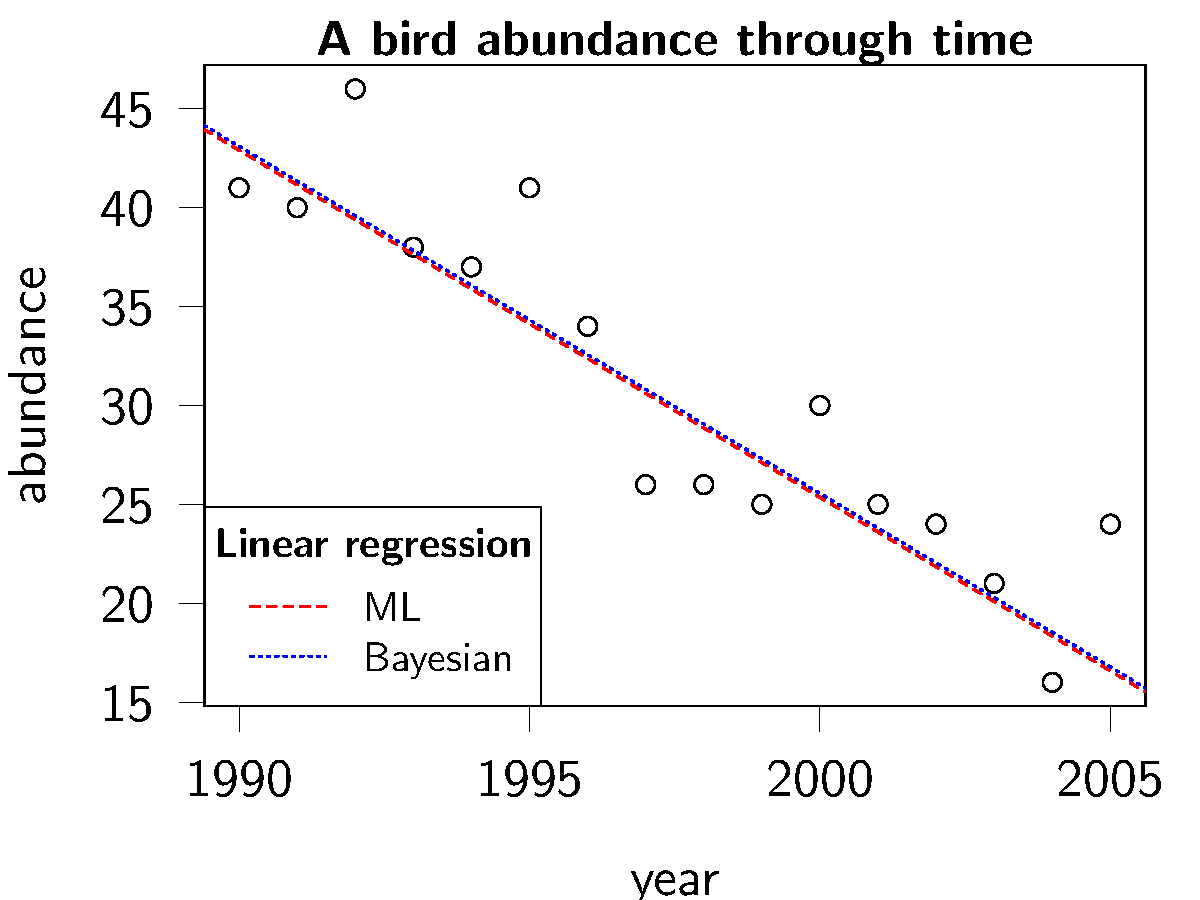
\includegraphics[width=0.67\textwidth,height=0.5\textwidth]{figure/tichodrome-1} 

\end{knitrout}
}

\only<2>{
\begin{alertblock}{Statistical models exist independently from inference method}
  \begin{itemize}
    \item Models are not Bayesian, nor frequentists (ML)
    \item In principle all can be fitted frequentist or Bayesian
    \item In general identical / very similar results
  \end{itemize}
\end{alertblock}
}
\end{frame}
%%%%%%%%%%%%

\begin{frame}{So why bother?}
  \textbf{Bayesian methods}
  \begin{itemize}[<+->]
    \item More (easily) flexible
    \item More intuitive interpretation
    \item Uncertainty propagation
    \item Easier to include missing values
    \item Incorporate previous knowledge
    \item The only feasible way for complex models
  \end{itemize}
\end{frame}
%%%%%%%%%%%

\begin{frame}{Today}
\large
  \begin{enumerate}
    \item Bayesian philosophy 101
    \item Fit your first Bayesian model
    \item MCMC in a nutshell
    \item The magic of the posterior
    \item Using priors
  \end{enumerate}
\pause
\textit{Convince you to come back for more}
\end{frame}
%%%%%%%%%%%


\begin{frame}{Bayesian philosophy 101}
  \centering \large{Is it raining outside?\\}
  \pause
  \centering \large{How many heads did I get?}
  \pause
  \begin{alertblock}{When you think Bayesian}
    \begin{itemize}
      \item You need a model
      \item Prior information may help
      \item Not one sure answer, only probabilities
    \end{itemize}
  \end{alertblock}
\end{frame}
%%%%%%%%%%%

\begin{frame}{Bayesian vs. Frequentist philosophies}

\textbf{\large Frequentist philosophy\\}
\textbf{Probability} = long run frequencies in fictuous populations\\
\uncover<2->{\textbf{Uncertainty} (p-value, CI, SE) = frequencies of data given parameter values\\}
\uncover<3->{\textbf{Unknown parameters} have \textbf{true, fixed,} values, generating data\\}

\bigskip

\textbf{\large Bayesian philosophy\\}
\textbf{Probability} = plausibility of a proposition \\
\uncover<2->{\textbf{Uncertainty} = probability of parameter values given data\\}
\uncover<3->{\textbf{Unknown parameters} have \textbf{probability distributions}, data are fixed\\}
\bigskip
\uncover<4->{\textbf{\textit{Enough blabla!}}}
\end{frame}
%%%%%%%%%%%

\section{Fit a Bayesian model in MCMCglmm}

\begin{frame}[fragile]{Fit Bayesian in R}



Load metabo data: metabolic rate and mass measured in 3 populations
\begin{knitrout}\small
\definecolor{shadecolor}{rgb}{0.843, 0.867, 0.922}\color{fgcolor}\begin{kframe}
\begin{alltt}
\hlstd{metabo} \hlkwb{<-} \hlkwd{read.csv}\hlstd{(}\hlstr{"metabo.csv"}\hlstd{)}
\end{alltt}
\end{kframe}
\end{knitrout}
\textbf{Metabolic rate differ among populations?}

\pause 

\texttt{install.packages("MCMCglmm")}

\begin{knitrout}\small
\definecolor{shadecolor}{rgb}{0.843, 0.867, 0.922}\color{fgcolor}\begin{kframe}
\begin{alltt}
\hlkwd{library}\hlstd{(MCMCglmm)}
\hlstd{m_pop} \hlkwb{<-} \hlkwd{MCMCglmm}\hlstd{(metabolism} \hlopt{~} \hlnum{1} \hlopt{+} \hlstd{pop,} \hlkwc{data} \hlstd{= metabo)}
\hlkwd{summary}\hlstd{(m_pop)}
\end{alltt}
\end{kframe}
\end{knitrout}

\end{frame}
%%%%%%%%%%%


\section{Closer look, and MCMC}

\begin{frame}[fragile]{The posterior distribution}
\begin{knitrout}\small
\definecolor{shadecolor}{rgb}{0.843, 0.867, 0.922}\color{fgcolor}\begin{kframe}
\begin{alltt}
\hlkwd{plot}\hlstd{(m_pop)}
\end{alltt}
\end{kframe}
\end{knitrout}

\pause

\begin{knitrout}\small
\definecolor{shadecolor}{rgb}{0.843, 0.867, 0.922}\color{fgcolor}\begin{kframe}
\begin{alltt}
\hlkwd{plot}\hlstd{(m_pop}\hlopt{$}\hlstd{Sol[,}\hlstr{"poppop2"}\hlstd{])}
\end{alltt}
\end{kframe}
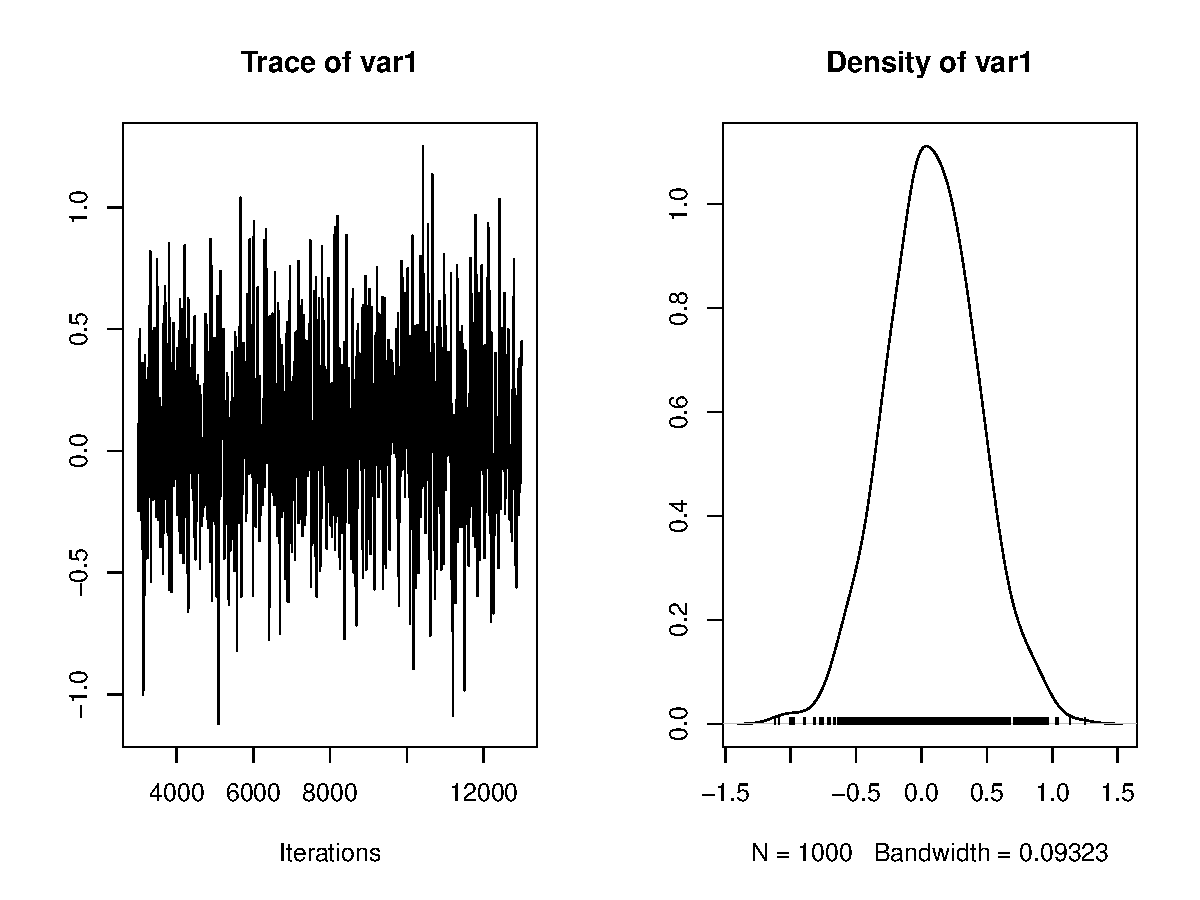
\includegraphics[width=0.67\textwidth,height=0.5\textwidth]{figure/unnamed-chunk-5-1} 

\end{knitrout}


\end{frame}
%%%%%%%%%%%

\begin{frame}[fragile]{The posterior distribution}

  \textbf{\large Posterior = Distribution of probability(Parameter $|$ Data)}
  \pause
  
  Approximated by Markov Chain Monte Carlo (MCMC) with Metropolis Hastings:\\
  
  \url{https://chi-feng.github.io/mcmc-demo/app.html?algorithm=RandomWalkMH&target=standard}
  

\end{frame}
%%%%%%%%%%%

\begin{frame}[fragile]{How many MCMC samples to approximate the posterior?}

MCMC parameters: \begin{itemize}
\item Number of iterations (nitt)
\item Discard N first iterations (burnin)
\item Save one iteration every N iterations (thin)
\end{itemize}

\begin{knitrout}\small
\definecolor{shadecolor}{rgb}{0.843, 0.867, 0.922}\color{fgcolor}\begin{kframe}
\begin{alltt}
\hlstd{m_pop_short} \hlkwb{<-} \hlkwd{MCMCglmm}\hlstd{(metabolism} \hlopt{~} \hlnum{1} \hlopt{+} \hlstd{pop,} \hlkwc{data} \hlstd{= metabo,}
                        \hlkwc{nitt} \hlstd{=} \hlnum{100}\hlstd{,} \hlkwc{burnin} \hlstd{=} \hlnum{0}\hlstd{,} \hlkwc{thin} \hlstd{=} \hlnum{10}\hlstd{)}
\hlkwd{plot}\hlstd{(m_pop_short)}

\hlstd{m_pop_long} \hlkwb{<-} \hlkwd{MCMCglmm}\hlstd{(metabolism} \hlopt{~} \hlnum{1} \hlopt{+} \hlstd{pop,} \hlkwc{data} \hlstd{= metabo,}
                        \hlkwc{nitt} \hlstd{=} \hlnum{100000}\hlstd{,} \hlkwc{burnin} \hlstd{=} \hlnum{0}\hlstd{,} \hlkwc{thin} \hlstd{=} \hlnum{10}\hlstd{)}
\hlkwd{plot}\hlstd{(m_pop_long)}
\end{alltt}
\end{kframe}
\end{knitrout}

\end{frame}
%%%%%%%%%%%

\begin{frame}[fragile]{That is fancy, but this model is not smart}
 
\begin{knitrout}\small
\definecolor{shadecolor}{rgb}{0.843, 0.867, 0.922}\color{fgcolor}\begin{kframe}
\begin{alltt}
 \hlkwd{MCMCglmm}\hlstd{(metabolism} \hlopt{~} \hlnum{1} \hlopt{+} \hlstd{pop,} \hlkwc{data} \hlstd{= metabo)}
\end{alltt}
\end{kframe}
\end{knitrout}

 \pause

\begin{knitrout}\small
\definecolor{shadecolor}{rgb}{0.843, 0.867, 0.922}\color{fgcolor}\begin{kframe}
\begin{alltt}
\hlstd{m_mpop} \hlkwb{<-} \hlkwd{MCMCglmm}\hlstd{(metabolism} \hlopt{~} \hlnum{1} \hlopt{+} \hlstd{mass} \hlopt{+} \hlstd{pop,} \hlkwc{data} \hlstd{= metabo)}
\hlkwd{summary}\hlstd{(m_mpop)}
\end{alltt}
\end{kframe}
\end{knitrout}
 
\end{frame}
%%%%%%%%%%%

\section{Posterior magic}

\begin{frame}[fragile]{Ask any question, get probabilities}

Default pMCMC = parameter estimates different from 0?
\begin{knitrout}\small
\definecolor{shadecolor}{rgb}{0.843, 0.867, 0.922}\color{fgcolor}\begin{kframe}
\begin{alltt}
\hlnum{2}\hlopt{*}\hlkwd{mean}\hlstd{(m_mpop}\hlopt{$}\hlstd{Sol[,}\hlstr{"poppop2"}\hlstd{]}\hlopt{<}\hlnum{0}\hlstd{)}
\end{alltt}
\begin{verbatim}
[1] 0.314
\end{verbatim}
\end{kframe}
\end{knitrout}


\pause

similar to frequentist p-value:
\begin{knitrout}\small
\definecolor{shadecolor}{rgb}{0.843, 0.867, 0.922}\color{fgcolor}\begin{kframe}
\begin{alltt}
\hlkwd{summary}\hlstd{(}\hlkwd{lm}\hlstd{(metabolism} \hlopt{~} \hlnum{1} \hlopt{+} \hlstd{mass} \hlopt{+} \hlstd{pop,} \hlkwc{data} \hlstd{= metabo))}\hlopt{$}\hlstd{coef}
\end{alltt}
\begin{verbatim}
             Estimate Std. Error   t value     Pr(>|t|)
(Intercept) 0.2431512 0.15235074  1.595996 1.225743e-01
mass        0.6521987 0.04121795 15.823173 7.334158e-15
poppop2     0.1053947 0.10333643  1.019918 3.171646e-01
poppop3     0.2175522 0.10940948  1.988422 5.738763e-02
\end{verbatim}
\end{kframe}
\end{knitrout}

In frequentist you are stuck with this, because only point estimate.
\textbf{In Bayesian, you can change the question, because you know probability of all possible values}

\end{frame}

\begin{frame}[fragile]{Ask any question, get probabilities}

Is the effect pop2 different from 0.1? from -0.2?
\begin{knitrout}\small
\definecolor{shadecolor}{rgb}{0.843, 0.867, 0.922}\color{fgcolor}\begin{kframe}
\begin{alltt}
\hlnum{2}\hlopt{*}\hlkwd{mean}\hlstd{(m_mpop}\hlopt{$}\hlstd{Sol[,}\hlstr{"poppop2"}\hlstd{]}\hlopt{<}\hlnum{0.1}\hlstd{)}
\end{alltt}
\begin{verbatim}
[1] 0.9
\end{verbatim}
\begin{alltt}
\hlnum{2}\hlopt{*}\hlkwd{mean}\hlstd{(m_mpop}\hlopt{$}\hlstd{Sol[,}\hlstr{"poppop2"}\hlstd{]}\hlopt{< -} \hlnum{0.2}\hlstd{)}
\end{alltt}
\begin{verbatim}
[1] 0.002
\end{verbatim}
\end{kframe}
\end{knitrout}

\pause

Probability slope of mass different from 0.75? from 1?\\

\end{frame}
%%%%%%%%%%%
\begin{frame}[fragile]{Ask any question, get probabilities}

Are the effects of pop2 and pop3 different?
\begin{knitrout}\small
\definecolor{shadecolor}{rgb}{0.843, 0.867, 0.922}\color{fgcolor}\begin{kframe}
\begin{alltt}
\hlstd{popdiff} \hlkwb{<-} \hlstd{m_mpop}\hlopt{$}\hlstd{Sol[,}\hlstr{"poppop2"}\hlstd{]} \hlopt{-} \hlstd{m_mpop}\hlopt{$}\hlstd{Sol[,}\hlstr{"poppop3"}\hlstd{]}
\hlkwd{plot}\hlstd{(popdiff)}
\end{alltt}
\end{kframe}
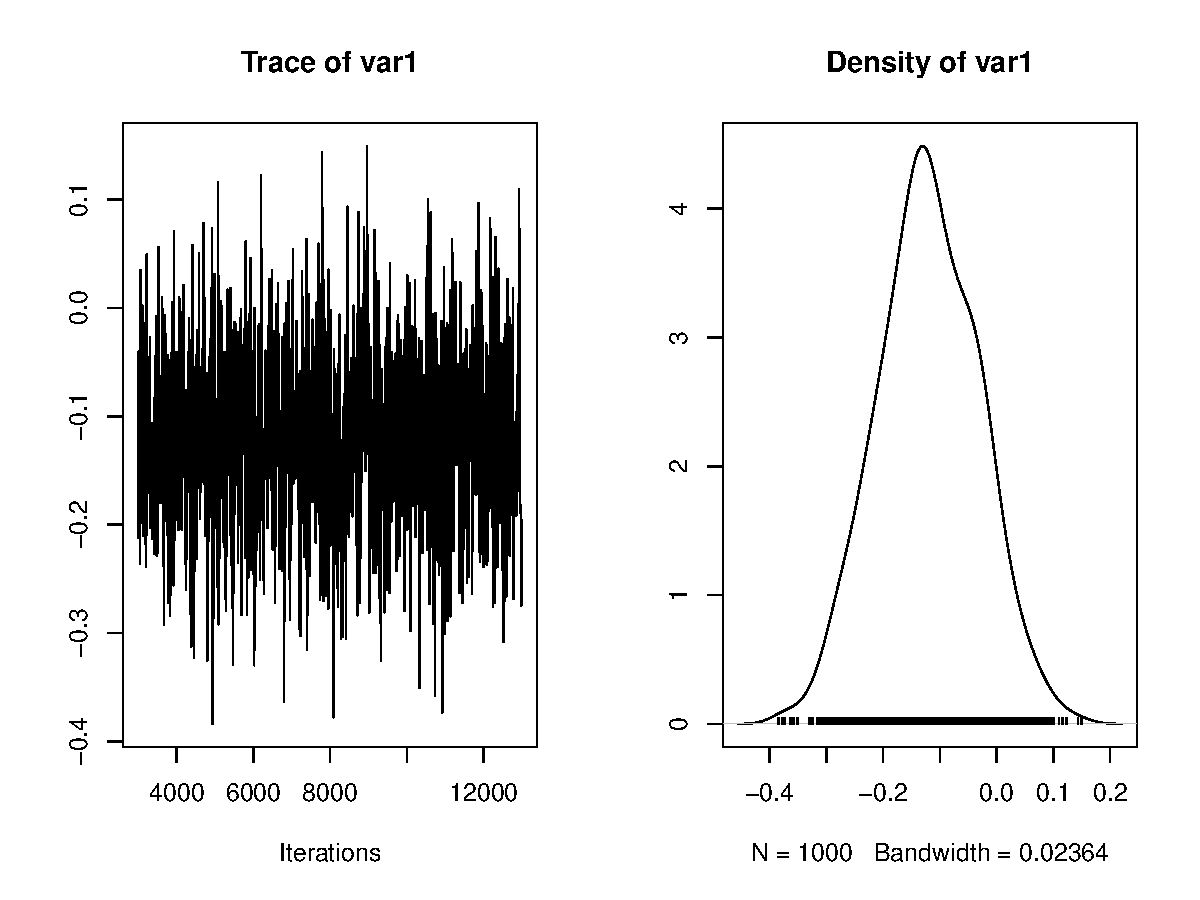
\includegraphics[width=0.67\textwidth,height=0.5\textwidth]{figure/unnamed-chunk-12-1} 

\end{knitrout}

\end{frame}
%%%%%%%%%%%

\begin{frame}[fragile]{Ask any question, get probabilities}

Is it likely that the effect of pop3 is more than twice that of pop2? More than half that of pop2?

\pause

Visualize the posterior of the exponential of the effect of mass plus 1.
\begin{knitrout}\small
\definecolor{shadecolor}{rgb}{0.843, 0.867, 0.922}\color{fgcolor}\begin{kframe}
\begin{alltt}
\hlkwd{plot}\hlstd{(}\hlkwd{exp}\hlstd{(m_mpop}\hlopt{$}\hlstd{Sol[,}\hlstr{"mass"}\hlstd{]} \hlopt{+} \hlnum{1}\hlstd{))}
\end{alltt}
\end{kframe}
\end{knitrout}

\end{frame}
%%%%%%%%%%%

\section{Using the prior}

\begin{frame}{Bayes theorem}

\large
  
  \begin{align*}
  \text{Posterior probability} &= \frac{\text{Likelihood} \times \text{Prior probability}}{\text{Probability of data}}\\
   \text{Posterior probability} & \text{ is proportional to } \text{Likelihood} \times \text{Prior probability}
  \end{align*}

Probability of data is unknown, but MCMC can sample in proportion of posterior probability, and probabilities sum to 1, hence we know
\pause
  \begin{align*}
    P(\theta | y) &= \frac{P( y | \theta) \times P(\theta)}{P(y)}\\
                  & \propto P( y | \theta) \times P(\theta)
  \end{align*}

\end{frame}
%%%%%%%%%%%

\begin{frame}{Flat prior}
\only<1>{
\begin{knitrout}\small
\definecolor{shadecolor}{rgb}{0.843, 0.867, 0.922}\color{fgcolor}
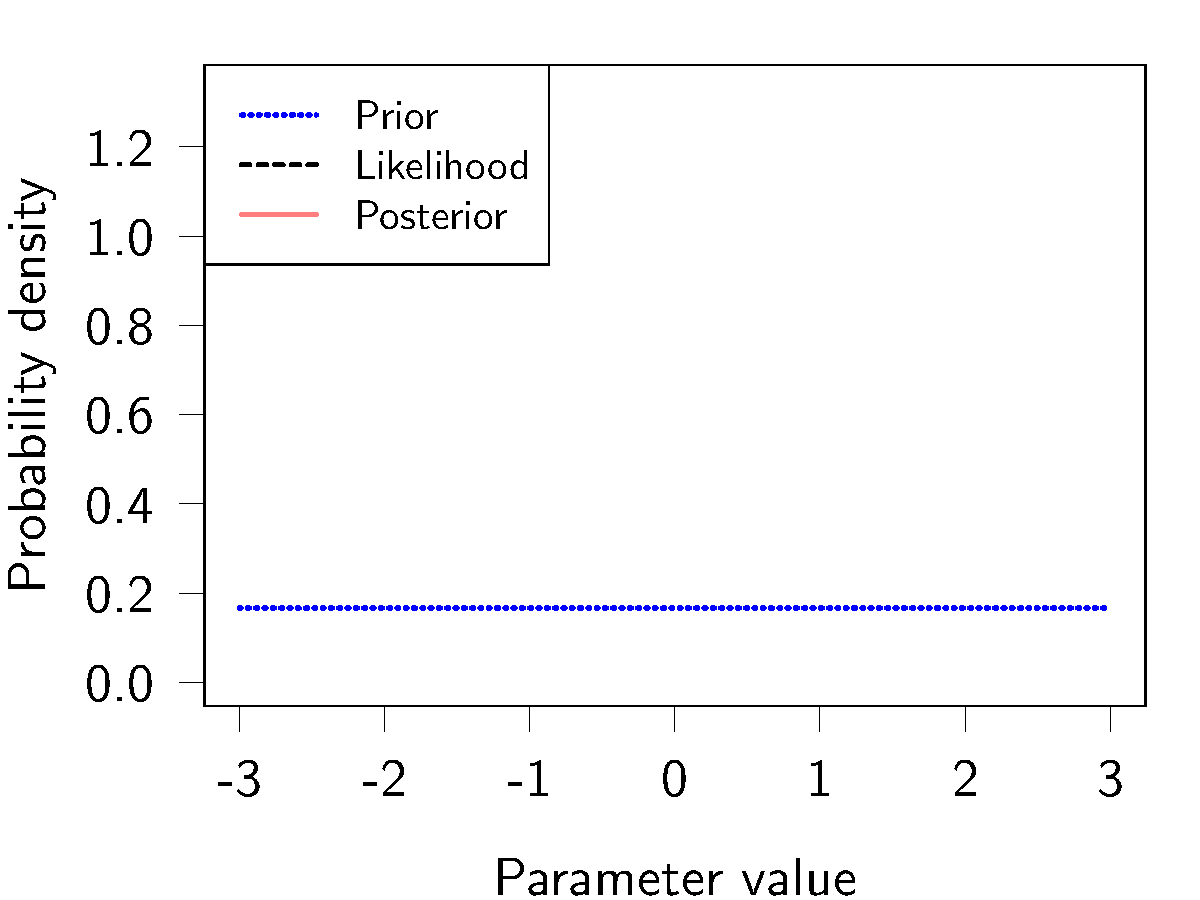
\includegraphics[width=0.67\textwidth,height=0.5\textwidth]{figure/flatprior1-1} 

\end{knitrout}
}

\only<2>{
\begin{knitrout}\small
\definecolor{shadecolor}{rgb}{0.843, 0.867, 0.922}\color{fgcolor}
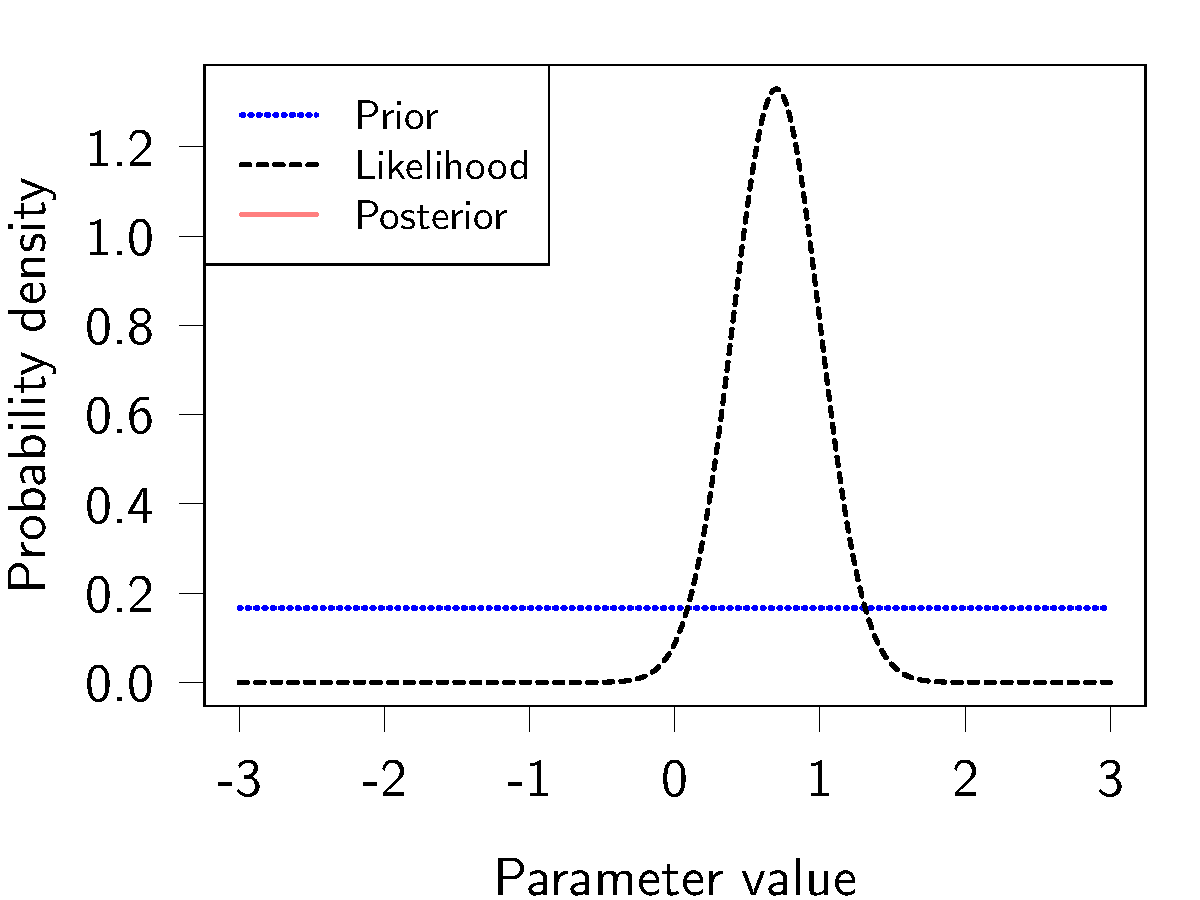
\includegraphics[width=0.67\textwidth,height=0.5\textwidth]{figure/flatprior2-1} 

\end{knitrout}
}

\only<3>{
\begin{knitrout}\small
\definecolor{shadecolor}{rgb}{0.843, 0.867, 0.922}\color{fgcolor}
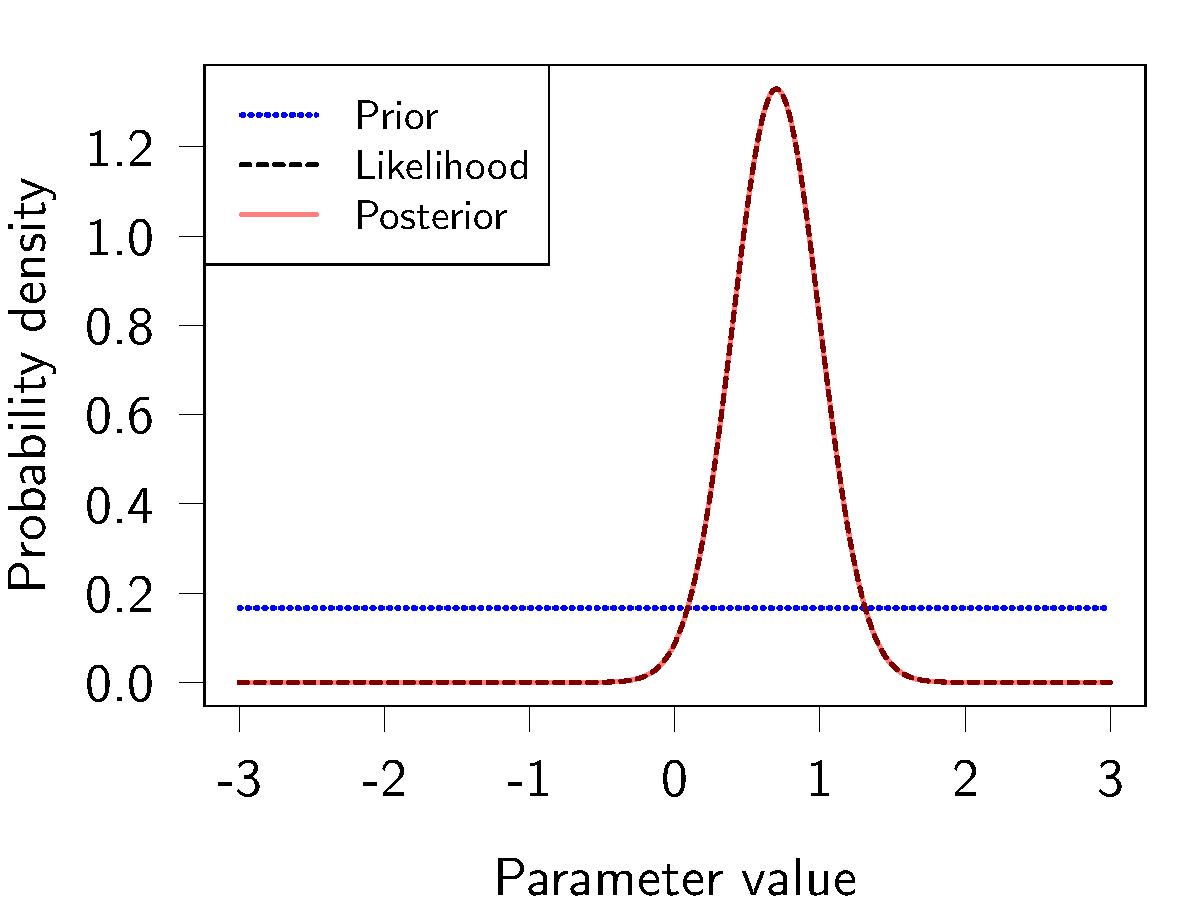
\includegraphics[width=0.67\textwidth,height=0.5\textwidth]{figure/flatprior3-1} 

\end{knitrout}
}

\end{frame}
%%%%%%%%%%%


\begin{frame}{Weakly informative prior}
\only<1>{
\begin{knitrout}\small
\definecolor{shadecolor}{rgb}{0.843, 0.867, 0.922}\color{fgcolor}
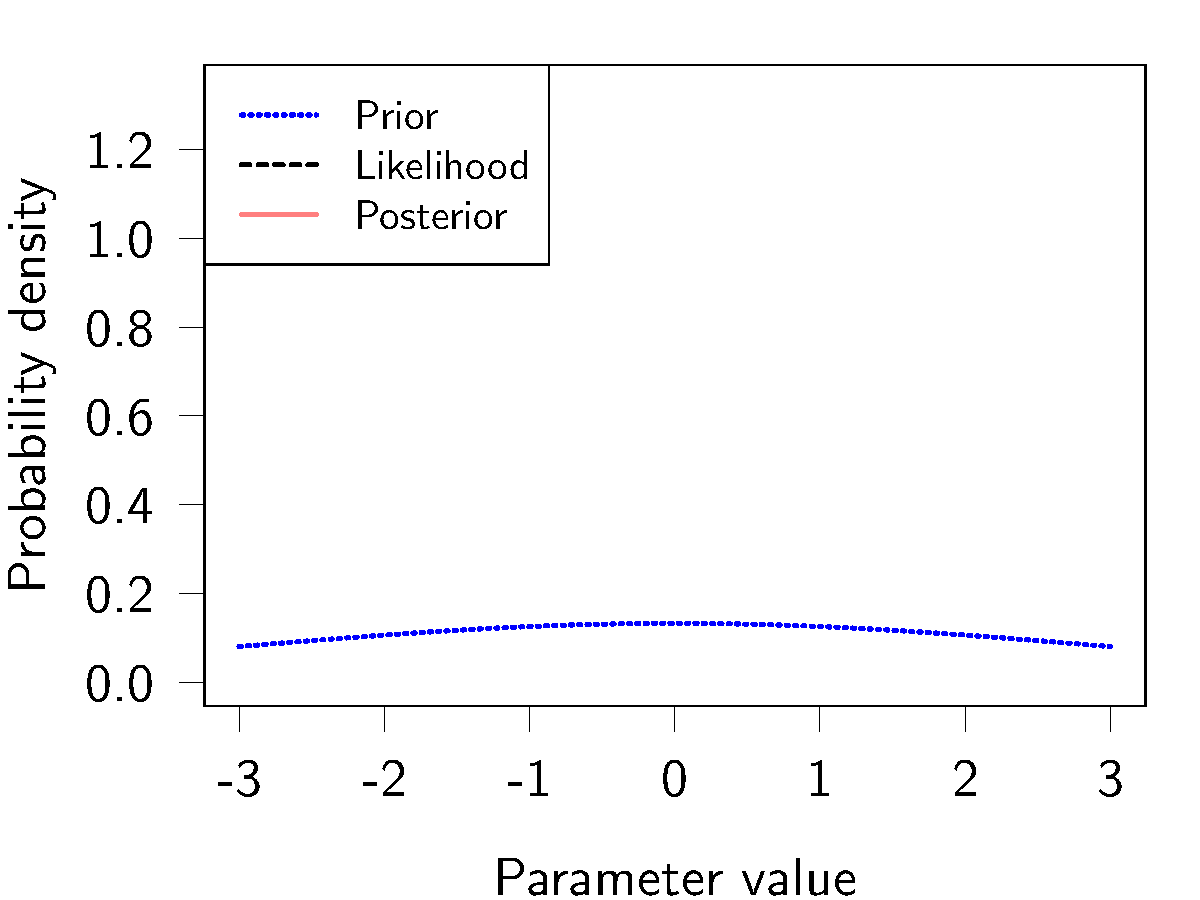
\includegraphics[width=0.67\textwidth,height=0.5\textwidth]{figure/normprior1-1} 

\end{knitrout}
}

\only<2>{
\begin{knitrout}\small
\definecolor{shadecolor}{rgb}{0.843, 0.867, 0.922}\color{fgcolor}
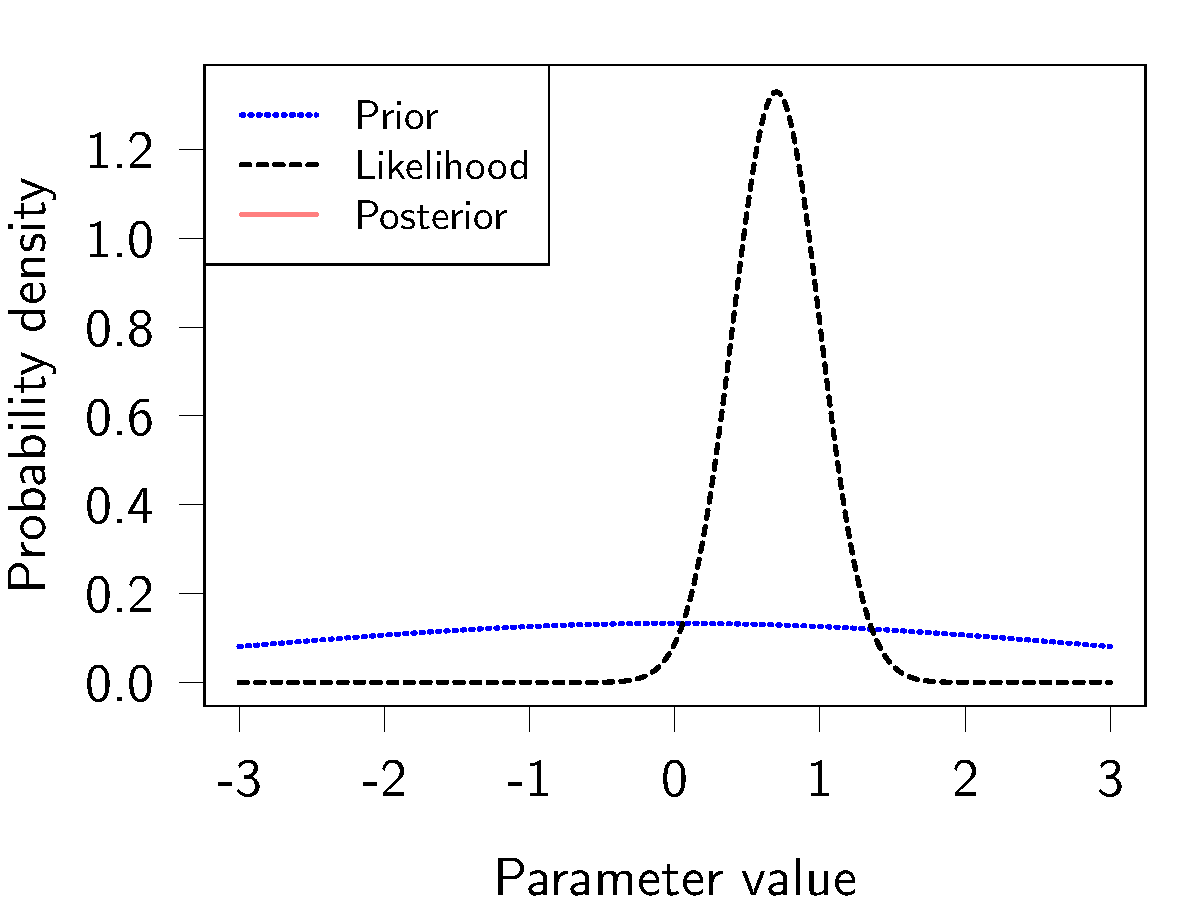
\includegraphics[width=0.67\textwidth,height=0.5\textwidth]{figure/normprior2-1} 

\end{knitrout}
}

\only<3>{
\begin{knitrout}\small
\definecolor{shadecolor}{rgb}{0.843, 0.867, 0.922}\color{fgcolor}
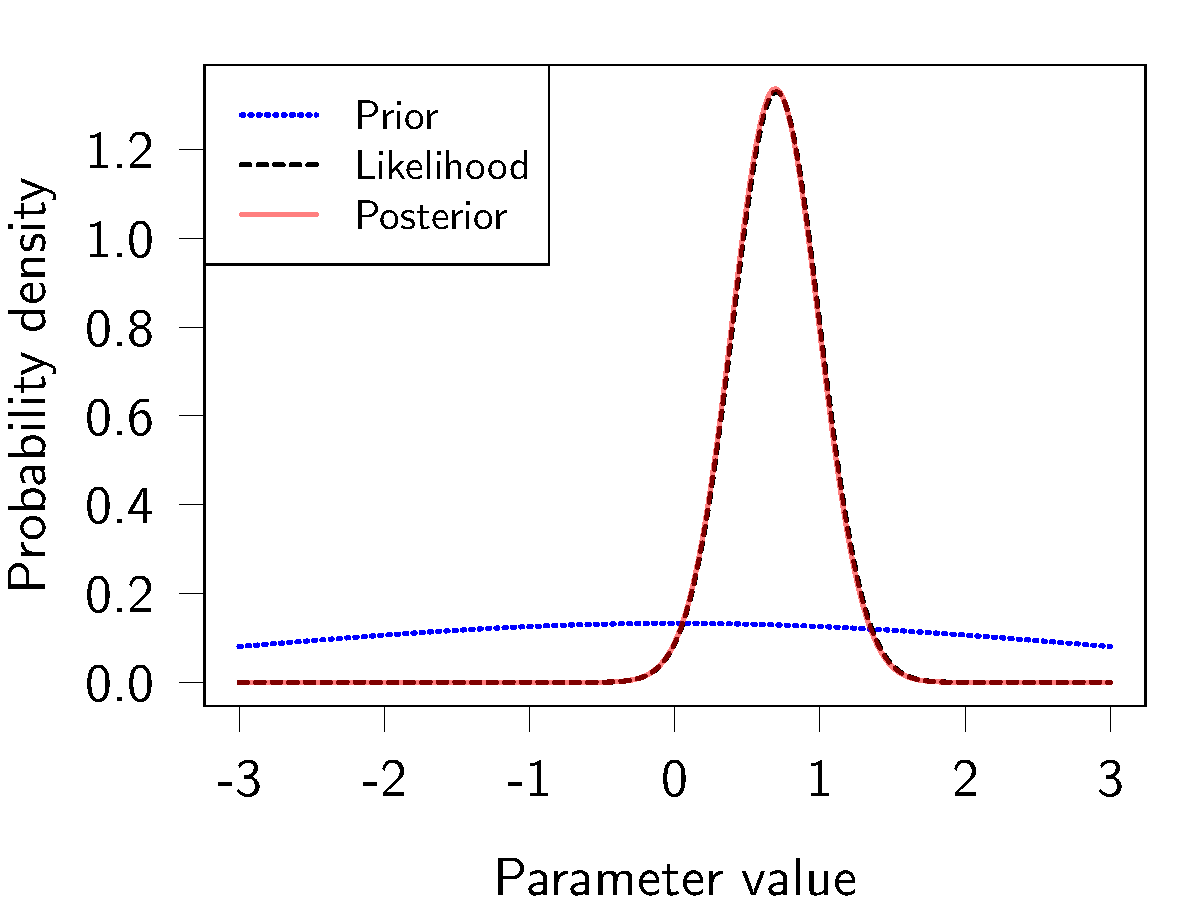
\includegraphics[width=0.67\textwidth,height=0.5\textwidth]{figure/normprior3-1} 

\end{knitrout}
}

\end{frame}
%%%%%%%%%%%

\begin{frame}{Strong prior}
\only<1>{
\begin{knitrout}\small
\definecolor{shadecolor}{rgb}{0.843, 0.867, 0.922}\color{fgcolor}
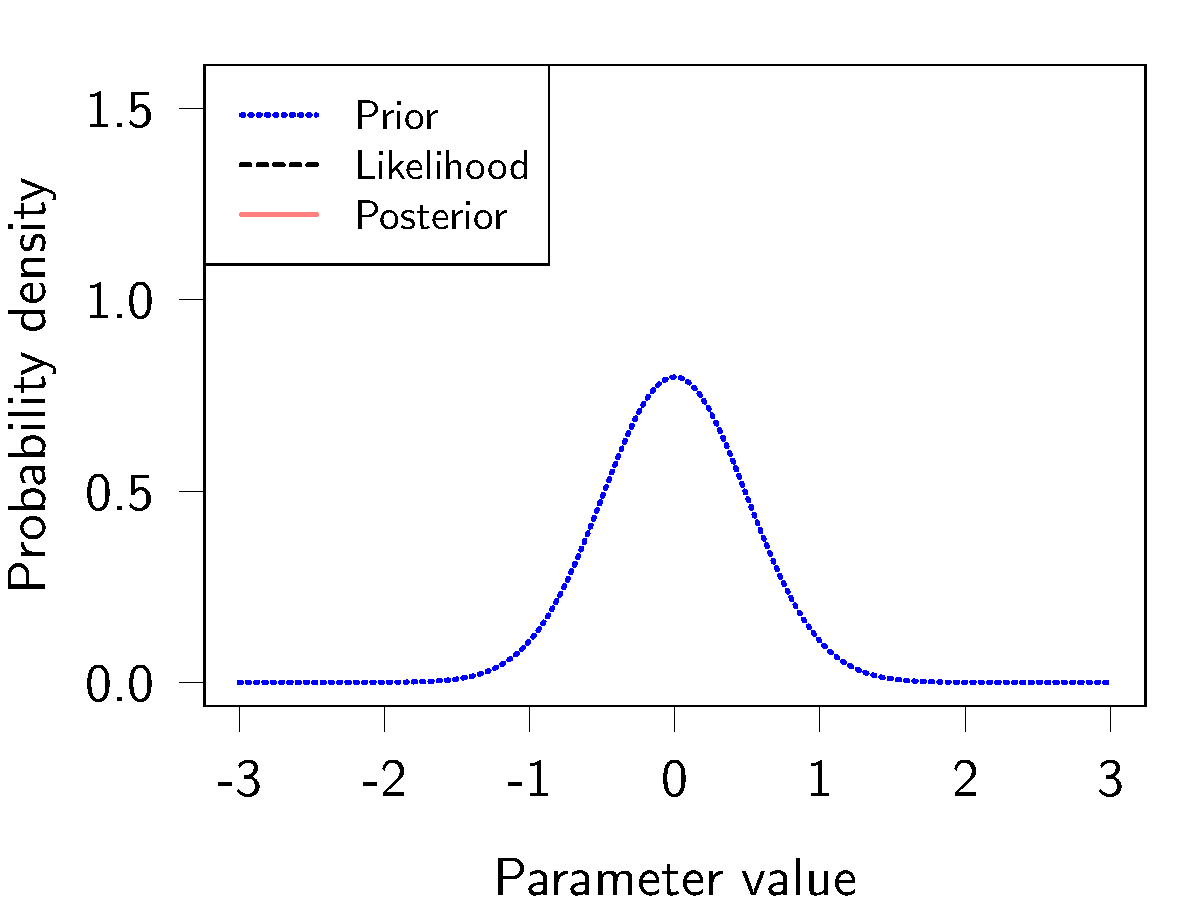
\includegraphics[width=0.67\textwidth,height=0.5\textwidth]{figure/strprior1-1} 

\end{knitrout}
}

\only<2>{
\begin{knitrout}\small
\definecolor{shadecolor}{rgb}{0.843, 0.867, 0.922}\color{fgcolor}
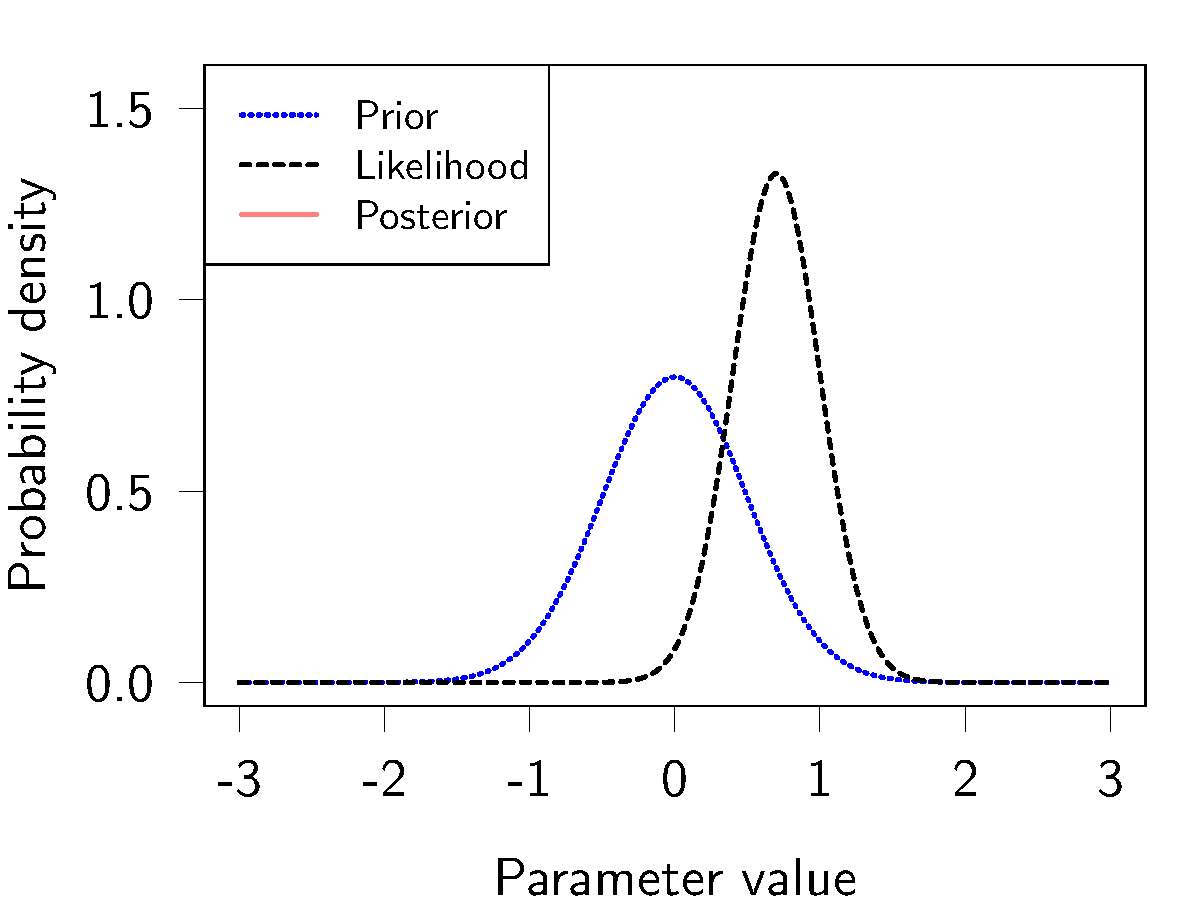
\includegraphics[width=0.67\textwidth,height=0.5\textwidth]{figure/strprior2-1} 

\end{knitrout}
}

\only<3>{
\begin{knitrout}\small
\definecolor{shadecolor}{rgb}{0.843, 0.867, 0.922}\color{fgcolor}
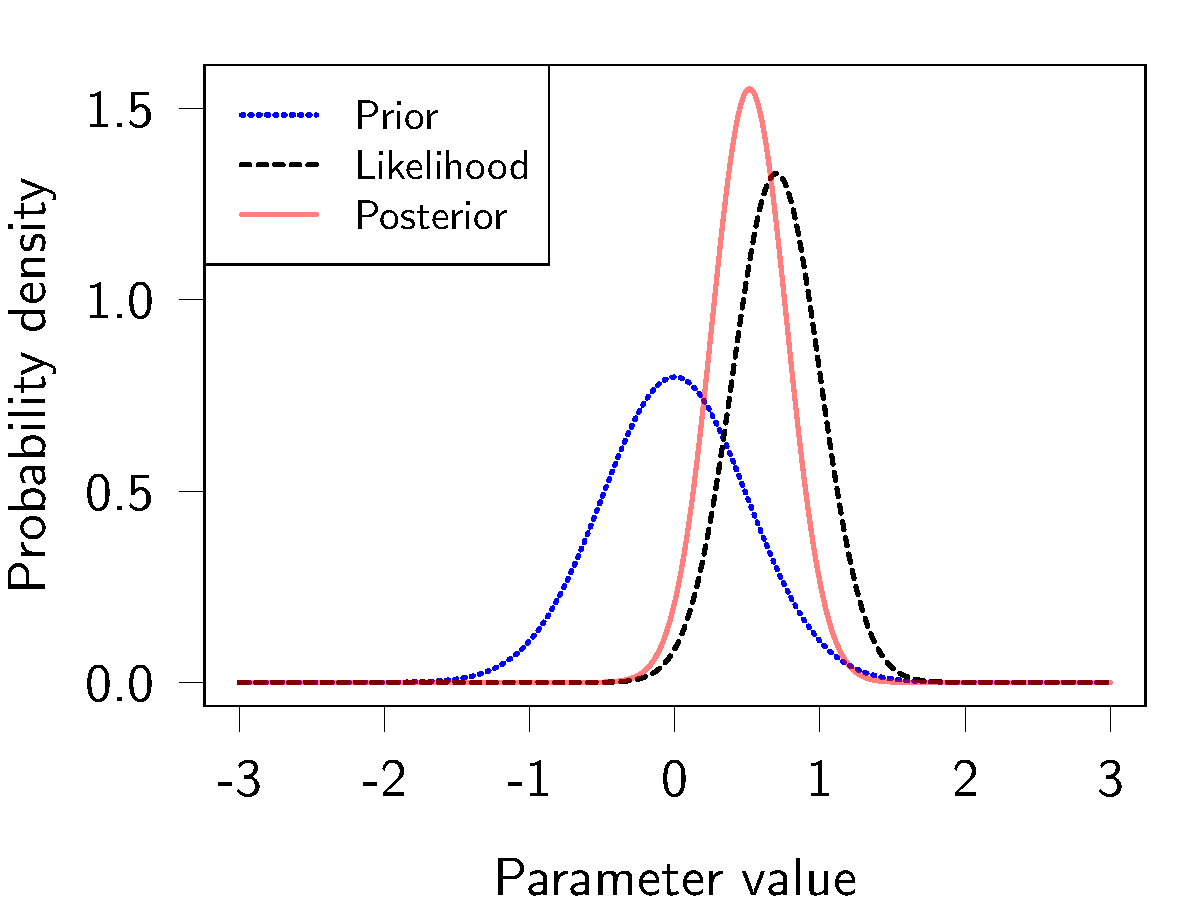
\includegraphics[width=0.67\textwidth,height=0.5\textwidth]{figure/strprior3-1} 

\end{knitrout}
}

\end{frame}
%%%%%%%%%%%

\begin{frame}{Strong prior}
\only<1>{
\begin{knitrout}\small
\definecolor{shadecolor}{rgb}{0.843, 0.867, 0.922}\color{fgcolor}
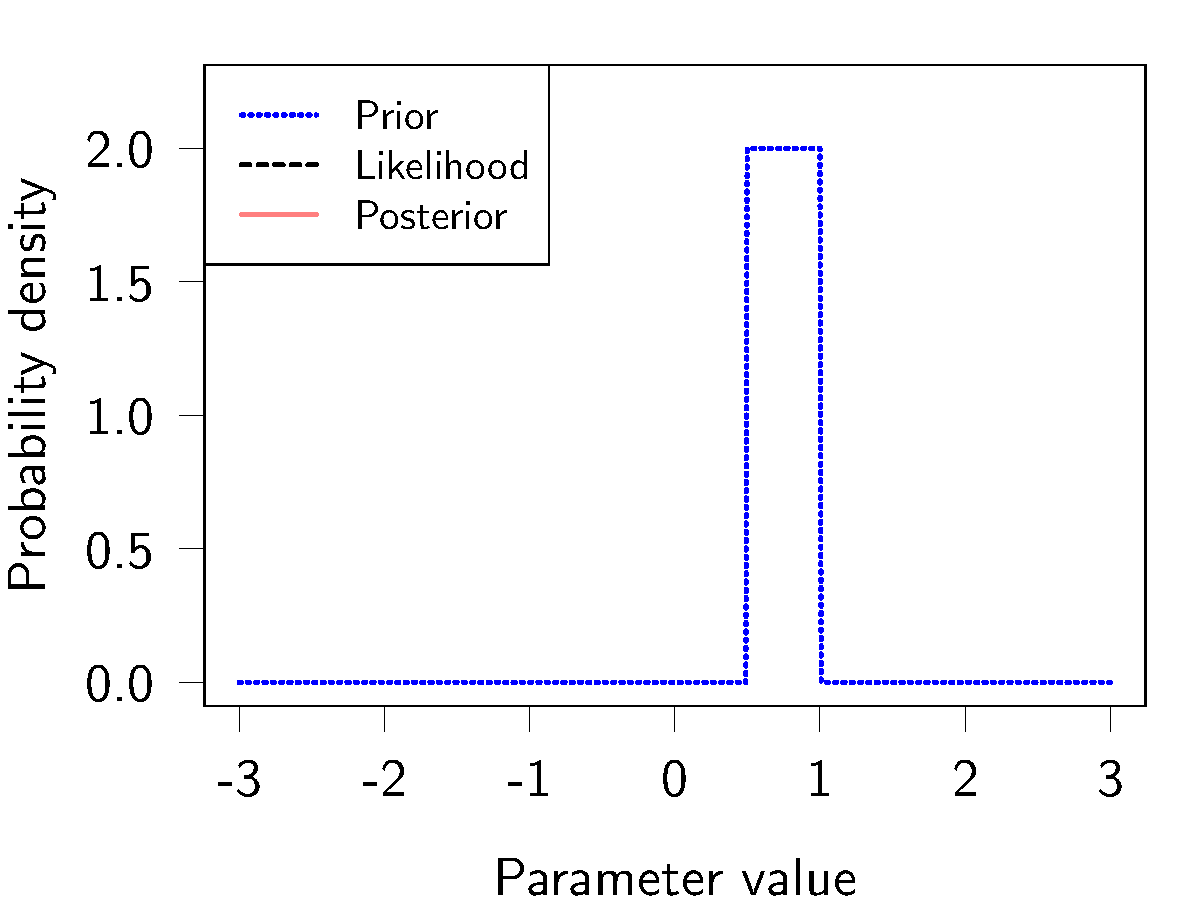
\includegraphics[width=0.67\textwidth,height=0.5\textwidth]{figure/trucprior1-1} 

\end{knitrout}
}

\only<2>{
\begin{knitrout}\small
\definecolor{shadecolor}{rgb}{0.843, 0.867, 0.922}\color{fgcolor}
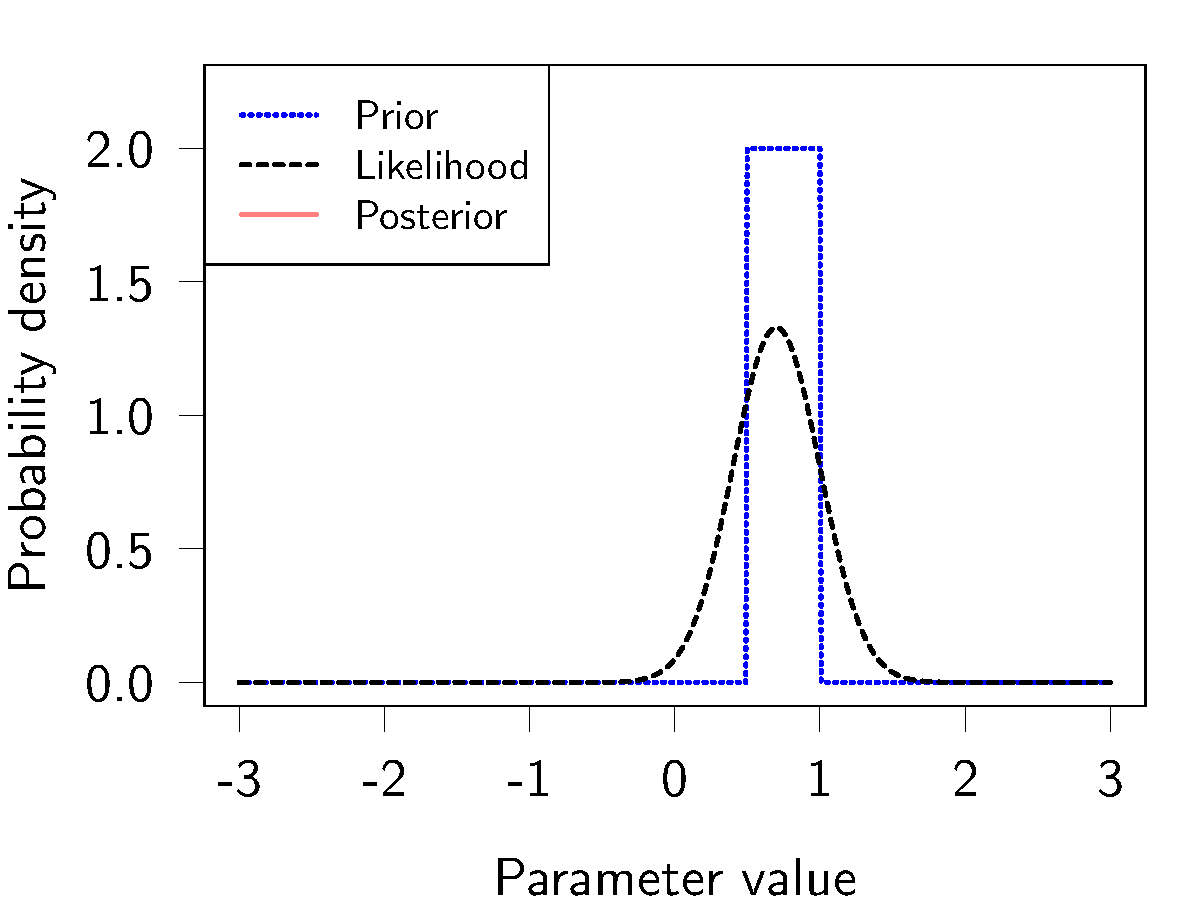
\includegraphics[width=0.67\textwidth,height=0.5\textwidth]{figure/trucprior2-1} 

\end{knitrout}
}

\only<3>{
\begin{knitrout}\small
\definecolor{shadecolor}{rgb}{0.843, 0.867, 0.922}\color{fgcolor}
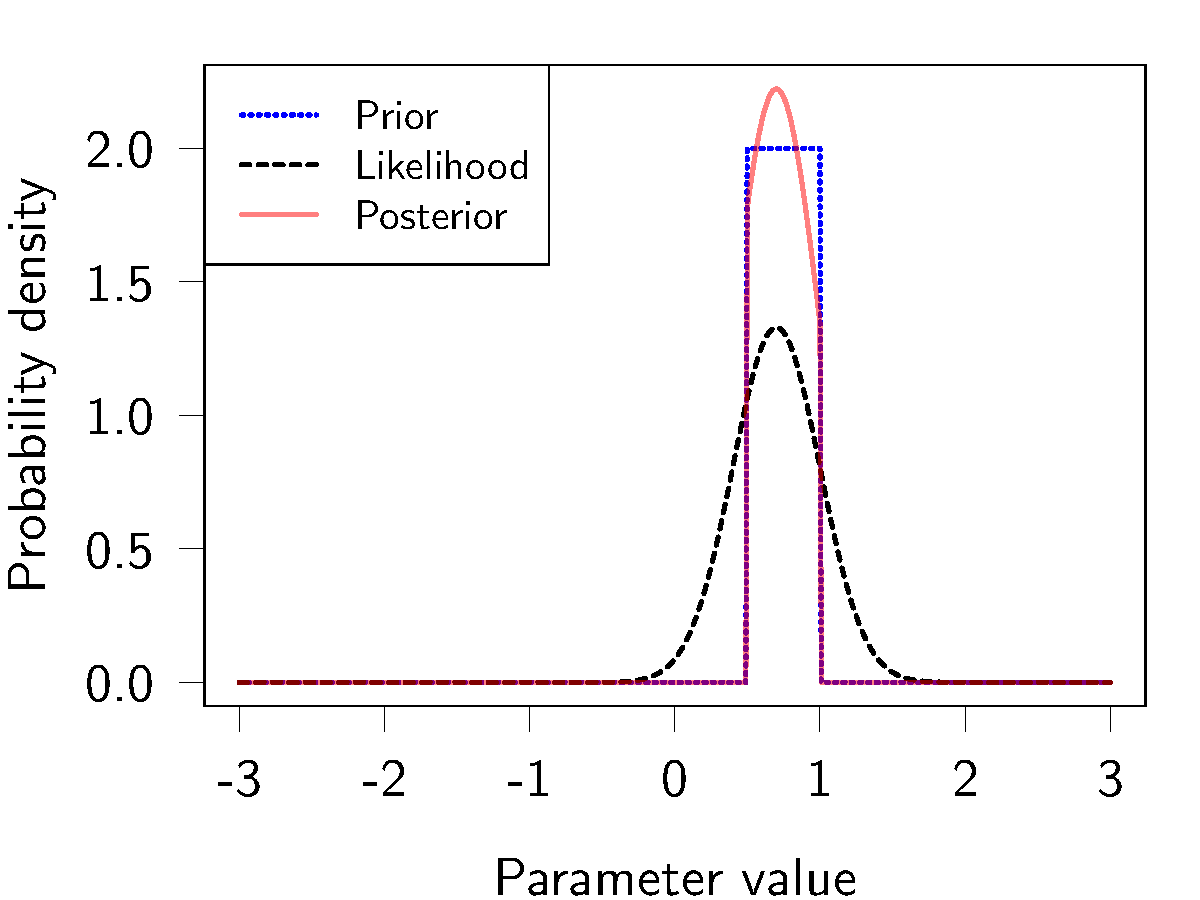
\includegraphics[width=0.67\textwidth,height=0.5\textwidth]{figure/trucprior3-1} 

\end{knitrout}
}

\end{frame}
%%%%%%%%%%%

\begin{frame}{In general you don't want prior to influence results}
\large
\alert{BUT, sometimes it will anyway. Need to be careful and check alternatives}

  \begin{exampleblock}{Sometimes informative priors are useful:}
    \begin{itemize}
      \item Correct for a well known nuisance parameter
      \item Missing data
      \item Avoid biologically impossible values
    \end{itemize}
  \end{exampleblock}

\end{frame}
%%%%%%%%%%%

\begin{frame}[fragile]{Change the prior in MCMCglmm}

Fixed effect priors follow normal distribution. Default mean = 0, variances = $10^{10}$, covariances = 0; almost flat:

\begin{knitrout}\small
\definecolor{shadecolor}{rgb}{0.843, 0.867, 0.922}\color{fgcolor}\begin{kframe}
\begin{alltt}
\hlstd{priorsamp} \hlkwb{<-} \hlkwd{rnorm}\hlstd{(}\hlkwc{n} \hlstd{=} \hlnum{10000000}\hlstd{,} \hlkwc{mean} \hlstd{=} \hlnum{0}\hlstd{,} \hlkwc{sd} \hlstd{=} \hlkwd{sqrt}\hlstd{(}\hlnum{10}\hlopt{^}\hlnum{10}\hlstd{))}
\hlkwd{plot}\hlstd{(}\hlkwd{density}\hlstd{(priorsamp),} \hlkwc{xlim}\hlstd{=}\hlkwd{c}\hlstd{(}\hlopt{-}\hlnum{100}\hlstd{,} \hlnum{100}\hlstd{))}
\end{alltt}
\end{kframe}
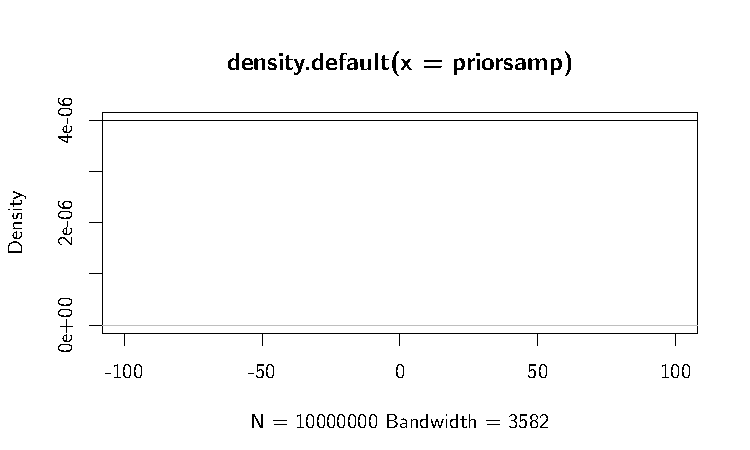
\includegraphics[width=0.67\textwidth,height=0.5\textwidth]{figure/simpr-1} 

\end{knitrout}

\end{frame}
%%%%%%%%%%%

\begin{frame}[fragile]{Change the prior in MCMCglmm}
We know from other studies the effect of mass is exactly 0.75.
\begin{knitrout}\small
\definecolor{shadecolor}{rgb}{0.843, 0.867, 0.922}\color{fgcolor}\begin{kframe}
\begin{alltt}
\hlstd{varprior} \hlkwb{<-} \hlkwd{diag}\hlstd{(}\hlnum{4}\hlstd{)}\hlopt{*}\hlnum{10000}
\hlstd{varprior[}\hlnum{2}\hlstd{,}\hlnum{2}\hlstd{]} \hlkwb{<-} \hlnum{0.000001}
\hlstd{prior1} \hlkwb{<-} \hlkwd{list}\hlstd{(}\hlkwc{B}\hlstd{=} \hlkwd{list}\hlstd{(}\hlkwc{mu}\hlstd{=}\hlkwd{c}\hlstd{(}\hlnum{0}\hlstd{,}\hlnum{0.75}\hlstd{,}\hlnum{0}\hlstd{,}\hlnum{0}\hlstd{),} \hlkwc{V}\hlstd{=varprior))}
\hlstd{mp} \hlkwb{<-} \hlkwd{MCMCglmm}\hlstd{(metabolism} \hlopt{~} \hlnum{1} \hlopt{+} \hlstd{mass} \hlopt{+} \hlstd{pop,} \hlkwc{data} \hlstd{= metabo,}
               \hlkwc{prior} \hlstd{= prior1)}
\hlkwd{summary}\hlstd{(mp)}
\end{alltt}
\end{kframe}
\end{knitrout}

\end{frame}
%%%%%%%%%%%

\begin{frame}[fragile]{Change the prior in MCMCglmm}
We know from other studies the effect of mass is exactly 0.75.
Another study has estimated the effect of pop2 to 0.15, with standard error of 0.01
\begin{knitrout}\small
\definecolor{shadecolor}{rgb}{0.843, 0.867, 0.922}\color{fgcolor}\begin{kframe}
\begin{alltt}
\hlstd{varprior} \hlkwb{<-} \hlkwd{diag}\hlstd{(}\hlnum{4}\hlstd{)}\hlopt{*}\hlnum{10000}
\hlstd{varprior[}\hlnum{2}\hlstd{,}\hlnum{2}\hlstd{]} \hlkwb{<-} \hlnum{0.000001}
\hlstd{varprior[}\hlnum{3}\hlstd{,}\hlnum{3}\hlstd{]} \hlkwb{<-} \hlnum{0.01}\hlopt{^}\hlnum{2}
\hlstd{prior2} \hlkwb{<-} \hlkwd{list}\hlstd{(}\hlkwc{B}\hlstd{=} \hlkwd{list}\hlstd{(}\hlkwc{mu}\hlstd{=}\hlkwd{c}\hlstd{(}\hlnum{0}\hlstd{,}\hlnum{0.75}\hlstd{,}\hlnum{0.15}\hlstd{,}\hlnum{0}\hlstd{),} \hlkwc{V}\hlstd{=varprior))}
\hlstd{mp2} \hlkwb{<-} \hlkwd{MCMCglmm}\hlstd{(metabolism} \hlopt{~} \hlnum{1} \hlopt{+} \hlstd{mass} \hlopt{+} \hlstd{pop,} \hlkwc{data} \hlstd{= metabo,}
                \hlkwc{prior} \hlstd{= prior2)}
\hlkwd{summary}\hlstd{(mp2)}
\end{alltt}
\end{kframe}
\end{knitrout}
\end{frame}
%%%%%%%%%%%


\begin{frame}{Some models much easier in Bayesian}
\textbf{Missing data in a predictor with a trend\\}
\pause
Missing data in temperarture you want to use to predict Survival at the end of time serie
\begin{knitrout}\small
\definecolor{shadecolor}{rgb}{0.843, 0.867, 0.922}\color{fgcolor}
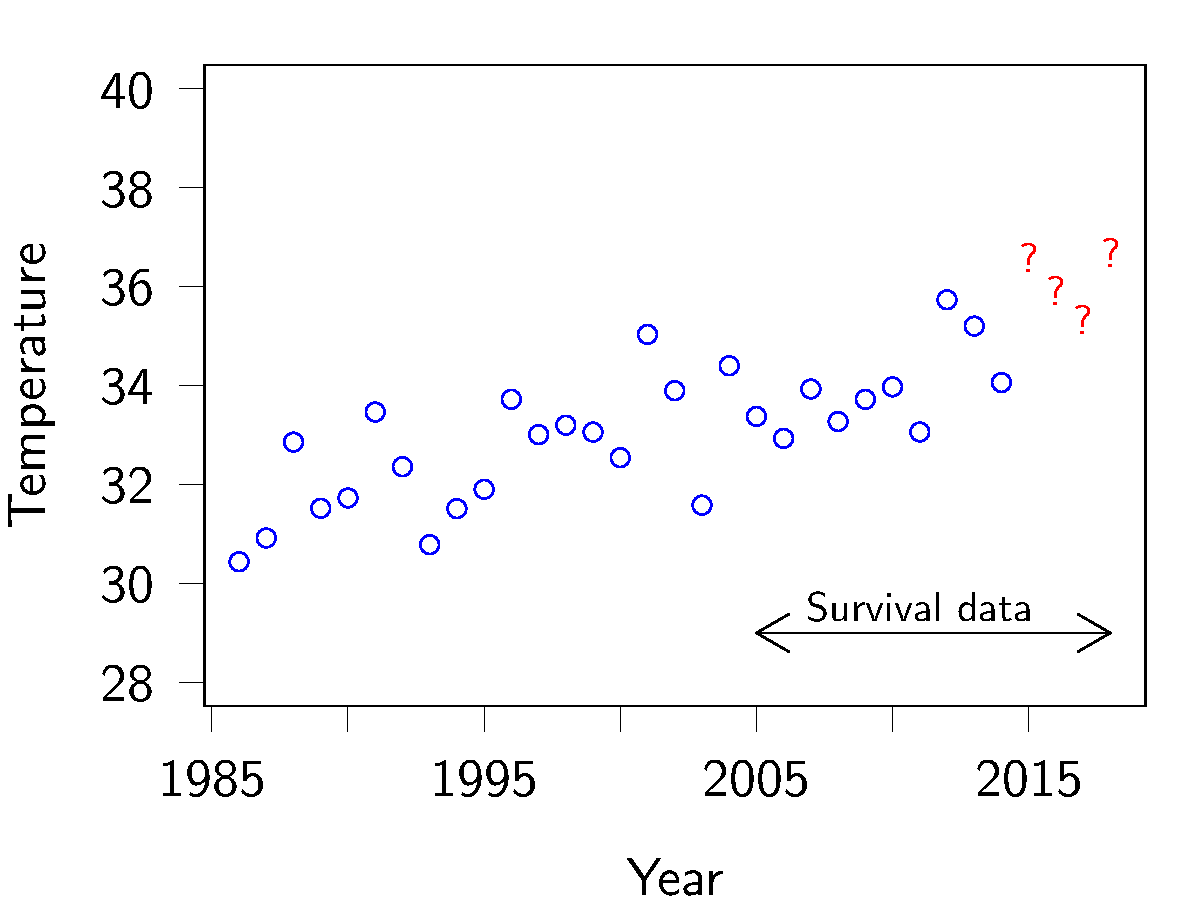
\includegraphics[width=0.67\textwidth,height=0.5\textwidth]{figure/tempmiss-1} 

\end{knitrout}

\end{frame}
%%%%%%%%%%%


\begin{frame}{Some models much easier in Bayesian}
Missing data in a predictor with a trend\\
\textbf{Combining information from different sources in a single model\\}
\pause

\begin{enumerate}[<+->]
  \item Fit individual growth curves to sparse mass data
  \item Estimate litter birth dates from estimate of mass$<$ birth mass, sibblings', time between litter
  \item Model snow cover 
  \item Model survival from mark-recapture data
  \item Estimate interaction snow cover by birth date on survival
  \item (plug in mean survival to a model of the number of individuals in population)
  \item (estimate how snow cover and population size impact vegetation growth)
  \item \dots
\end{enumerate}

\end{frame}
%%%%%%%%%%%

\begin{frame}{Want more?}

Two days on writing your own models in JAGS/STAN
  \begin{itemize}
    \item GLMMs
    \item Missing data
    \item Integrating multi-part models
    \item Priors, diagnostics, cool tools\dots
  \end{itemize}
  
\end{frame}
%%%%%%%%%%%

\end{document}
